\chapter{Energía y Hamiltoniano}

\lectureoverview{Primero precisaremos el significado de una simetría activa y repasaremos cómo las traslaciones y rotaciones generan el momento lineal y el momento angular. La ley de conservación que falta es la de la energía. Su simetría es la traslación en el tiempo, y la magnitud conservada es el Hamiltoniano \(H=\sum_i p_i\dot q_i-L\). La derivación también muestra exactamente cómo la dependencia explícita del tiempo transfiere energía entre un subsistema elegido y su entorno.}

\section{Preguntas antes del argumento formal}

Nos acercamos al mínimo absoluto de mecánica clásica necesario para los temas que siguen, aunque todavía queda mucha mecánica que merece la pena aprender. Antes de comenzar el argumento principal surgieron dos preguntas.

\begin{classroomqa}\audiencequestion{¿Qué libros son útiles después de este curso introductorio?\lecturetimestamp{00:00:36--00:02:13}}\lecturerresponse{La referencia avanzada de uso establecido es \emph{Classical Mechanics}, de Herbert Goldstein. El libro de Cornelius Lanczos sobre los principios variacionales de la mecánica es otra fuente pertinente. Una lista de lecturas para el curso resulta más útil que fingir que un solo profesor puede reseñar todos los textos disponibles.}\end{classroomqa}

La segunda pregunta recoge un momento de la historia de una medición que aún no se había resuelto. En 2011, el experimento OPERA había comunicado una llegada aparentemente anticipada de neutrinos enviados desde el CERN hasta Gran Sasso. La discrepancia comunicada era menor que la duración del pulso de protones utilizado para crear los neutrinos, por lo que el análisis temporal dependía de comparar los perfiles de los pulsos, en vez de etiquetar un neutrino en el momento de su emisión y reconocer la misma partícula al detectarla.

\begin{classroomqa}\audiencequestion{¿Se había resuelto el aparente resultado de neutrinos más rápidos que la luz?\lecturetimestamp{00:02:30--00:09:03}}\lecturerresponse{En ese momento no se justificaba ninguna conclusión. La forma del pulso del haz, el calentamiento del blanco y la sincronización requerían un examen técnico minucioso. Una propuesta especulativa consideraba el movimiento de un satélite GPS: en el sistema de referencia del satélite, la fuente y el detector se mueven mientras viajan las señales de sincronización, lo que produce correcciones del orden de decenas de nanosegundos. La estimación era interesante como ejercicio de orden de magnitud, pero no se presentó como un diagnóstico creíble del experimento. La contracción de Lorentz ordinaria a la velocidad pertinente era demasiado pequeña para explicar el efecto comunicado. Lo apropiado era esperar al análisis experimental.}\end{classroomqa}

\begin{figure}[htbp]\centering
  \includegraphics[width=0.78\textwidth]{lecture_05_figure_07.png}\caption{Esquema temporal en el sistema de referencia del satélite, comentado durante la pregunta histórica sobre la medición de neutrinos.}\lectureframe{00:06:30}\end{figure}

La discusión sobre la medición temporal no es necesaria para la mecánica que sigue. Sin embargo, sirve para recordar que una estimación de escala plausible no equivale a una explicación experimental establecida.

\section{Simetría activa y elección del sistema}

Volvamos al punto que quedó demasiado impreciso en la discusión anterior: ¿qué es exactamente una simetría? Consideremos una partícula sobre una recta y la instrucción \begin{equation}
  x\longrightarrow x+1.
  \label{eq:l5-shift-one}
\end{equation}. Hay dos maneras de entenderla. Una transformación \emph{pasiva} cambia las etiquetas de los puntos de la recta. Un punto que antes se llamaba \(x=0\) puede llamarse ahora \(x'=1\), pero la partícula no se ha movido. Una transformación \emph{activa} mantiene fijas las etiquetas y mueve la propia partícula de \(x\) a \(x+1\). Solo la segunda operación cambia su posición respecto de un potencial externo.

\begin{figure}[htbp]\centering
  \includegraphics[width=0.82\textwidth]{lecture_05_figure_08.png}\caption{La regla \(x\mapsto x+1\), la recta de coordenadas fija y un potencial externo permiten distinguir el movimiento activo de un mero cambio pasivo de etiquetas.}\lectureframe{00:11:20}\end{figure}

\begin{classroomqa}\audiencequestion{Si al mover la partícula cambia su energía potencial, ¿se está excluyendo del sistema la fuente de ese potencial?\lecturetimestamp{00:12:19--00:14:18}}\lecturerresponse{Exactamente. Al hablar de ``una partícula en un potencial'', dividimos el mundo entre la partícula y un entorno pesado, como la Tierra, que produce \(V(x)\). La Tierra sí retrocede, pero su enorme masa hace que ese retroceso sea despreciable en esta aproximación. Mover la partícula respecto de la Tierra fija puede cambiar \(V\); trasladar conjuntamente la partícula y la Tierra no lo haría.}\end{classroomqa}

\begin{classroomqa}\audiencequestion{En el ejemplo anterior de rotación, ¿también cambiaban las velocidades, además de las posiciones?\lecturetimestamp{00:14:26--00:15:29}}\lecturerresponse{Sí. Una rotación activa rígida actúa sobre toda la historia, no solo sobre una posición instantánea. Se rotan tanto las posiciones como los vectores velocidad. En cambio, una traslación constante aplicada en todo instante cambia \(x\), pero deja \(\dot x\) sin cambios.}\end{classroomqa}

La distinción entre sistema y entorno volverá a aparecer en dos ocasiones: cuando un aparato cuya evolución depende del tiempo intercambie energía con un subsistema, y cuando la fricción macroscópica oculte energía en un movimiento microscópico no observado.

\section{Desplazamientos infinitesimales en el espacio de configuraciones}

Una configuración de un sistema mecánico general es un punto del espacio de coordenadas generalizadas \(q_i\). Una transformación activa infinitesimal desplaza cada configuración posible a otra cercana. Escribimos \begin{equation}
  \delta q_i=\epsilon f_i(q),
  \label{eq:l5-general-transformation}
\end{equation}, donde las funciones \(f_i\) especifican un campo de desplazamientos fijo en el espacio de configuraciones. Pueden depender de todas las coordenadas, y algunas pueden anularse. El factor común \(\epsilon\) es pequeño; separa el tamaño del paso de la forma de la transformación.

\begin{figure}[htbp]\centering
  \includegraphics[width=0.75\textwidth]{lecture_05_figure_09.png}\caption{Un vector de desplazamiento asociado a cada punto del espacio de configuraciones.}\lectureframe{00:16:50}\end{figure}

\begin{figure}[htbp]\centering
  \includegraphics[width=0.80\textwidth]{lecture_05_figure_10.png}\caption{La transformación infinitesimal dependiente de las coordenadas \(\delta q_i=\epsilon f_i(q)\).}\lectureframe{00:18:00}\end{figure}

La regla en sí no depende explícitamente del tiempo. Por tanto, su acción sobre las velocidades es \begin{equation}
  \delta\dot q_i=\frac{d}{dt}(\delta q_i)
  =\epsilon\sum_j\frac{\partial f_i}{\partial q_j}\dot q_j.
  \label{eq:l5-velocity-variation}
\end{equation}. Para una traslación, \(f_x=1\), de modo que \(\delta\dot x=0\). En una rotación, \(f_i\) depende de la posición, y la velocidad cambia.

\begin{classroomqa}\audiencequestion{¿El último factor pequeño de \(\delta q_i=\epsilon f_i(q)\) es la misma constante en todos los puntos?\lecturetimestamp{00:19:58--00:20:51}}\lecturerresponse{Sí. La constante única \(\epsilon\) es un recurso de notación que hace que todos los cambios de coordenadas sean de primer orden en la misma cantidad pequeña. Las funciones \(f_i(q)\), no \(\epsilon\), contienen la dependencia espacial y no tienen por qué ser pequeñas.}\end{classroomqa}

\section{¿Qué hace que la transformación sea una simetría?}

En general, una transformación activa cambia la energía potencial. También puede cambiar la energía cinética. En coordenadas curvilíneas, el término cinético tiene la forma \begin{equation}
  T=\frac12\sum_{i,j}g_{ij}(q)\dot q_i\dot q_j,
  \label{eq:l5-kinetic-metric}
\end{equation}, por lo que un desplazamiento en el espacio de configuraciones puede cambiar sus coeficientes. El término familiar \(r^2\dot\theta^2\) en coordenadas polares es el ejemplo más sencillo.

Aquí, una transformación es una simetría cuando el \emph{Lagrangiano completo} no experimenta ningún cambio de primer orden: \begin{equation}
  \delta L=O(\epsilon^2),
  \label{eq:l5-symmetry-condition}
\end{equation}. Esto debe cumplirse en todos los puntos del espacio de configuraciones, no solo en la configuración que ocupa una solución particular.

Por ejemplo, bajo \(x\mapsto x+\epsilon\), \begin{equation}
  \delta V=\frac{\partial V}{\partial x}\epsilon.
  \label{eq:l5-potential-variation}
\end{equation}. Si esto se anula para todo \(x\) posible, entonces \(\partial V/\partial x=0\): el potencial es independiente de \(x\). Si permanece invariante bajo traslaciones en todas las direcciones espaciales, es constante.

\begin{figure}[htbp]\centering
  \includegraphics[width=0.80\textwidth]{lecture_05_figure_11.png}\caption{Una traslación en \(x\), comprobada con respecto a un potencial \(V(y)\) independiente de \(x\).}\lectureframe{00:23:40}\end{figure}

Para una familia suave de un parámetro, que el cambio de primer orden se anule en todos los puntos nos permite componer pasos infinitesimales hasta obtener una simetría finita.

\begin{classroomqa}\audiencequestion{¿Deben permanecer invariantes por separado la energía cinética y la potencial?\lecturetimestamp{00:24:44--00:25:33}}\lecturerresponse{No. Solo debe ser invariante el Lagrangiano total. Algunos Lagrangianos contienen términos mixtos de coordenadas-- y velocidades y no admiten una separación útil en \(T\) y \(V\), de modo que quizá ni siquiera tenga sentido preguntar por la invariancia por separado.}\end{classroomqa}

\begin{classroomqa}\audiencequestion{¿«Sin cambio»``'' significa que no hay cambio exactamente, o solo que el cambio es lo bastante pequeño como para despreciarlo?\lecturetimestamp{00:25:34--00:28:59}}\lecturerresponse{Para una transformación infinitesimal, significa que no hay ningún término proporcional a \(\epsilon\). En el cálculo local se descartan los términos de orden \(\epsilon^2\). Como la condición de primer orden se cumple en todos los puntos de la órbita de un parámetro, repetir el paso local produce la invariancia finita.}\end{classroomqa}

\section{Recuperación del momento lineal y el momento angular}

Para las simetrías puntuales exactas e independientes del tiempo que estamos considerando, el resultado demostrado anteriormente es \begin{equation}
  Q=\sum_i p_i f_i(q),
  \qquad
  p_i=\frac{\partial L}{\partial\dot q_i},
  \qquad
  \dot Q=0.
  \label{eq:l5-noether-charge}
\end{equation}. El factor \(\epsilon\) no forma parte de \(Q\); solo mide cuánto avanzamos a lo largo de la órbita de simetría.

\begin{figure}[htbp]\centering
  \includegraphics[width=0.82\textwidth]{lecture_05_figure_12.png}\caption{Desplazamiento infinitesimal general y carga de Noether conservada.}\lectureframe{00:30:00}\end{figure}

Para una traslación en \(x\), \(f_x=1\) y \(Q=p_x\). La invariancia completa frente a las traslaciones implica la conservación de las tres componentes del momento lineal. Para muchas partículas que interactúan, la simetría traslada todas las partículas conjuntamente, por lo que \begin{equation}
  \mathbf P=\sum_a\mathbf p_a
  \label{eq:l5-total-momentum}
\end{equation} se conserva si las interacciones dependen solo de las posiciones relativas. Mover una partícula respecto de las demás no es la simetría.

\begin{figure}[htbp]\centering
  \includegraphics[width=0.80\textwidth]{lecture_05_figure_13.png}\caption{Una traslación común implica la conservación del momento lineal total, componente a componente.}\lectureframe{00:32:50}\end{figure}

Para una rotación infinitesimal en el plano \(x\)-\(y\), elijamos la orientación \begin{equation}
  \delta x=-y\epsilon,
  \qquad
  \delta y=x\epsilon.
  \label{eq:l5-planar-rotation}
\end{equation}. El radio se conserva, porque \begin{equation}
  \delta(x^2+y^2)
  =2x\delta x+2y\delta y=0.
  \label{eq:l5-radius-invariance}
\end{equation}.

\begin{figure}[htbp]\centering
  \includegraphics[width=0.76\textwidth]{lecture_05_figure_14.png}\caption{Geometría y fórmula en coordenadas de una rotación plana infinitesimal.}\lectureframe{00:35:05}\end{figure}

Al derivar la ec.~\eqref{eq:l5-planar-rotation}, las velocidades también se rotan. Así, \(\dot x^2+\dot y^2\) es invariante, y un potencial central \(V(\sqrt{x^2+y^2})\) deja inalterado el Lagrangiano completo. La carga es \begin{equation}
  Q=-yp_x+xp_y=(\mathbf r\times\mathbf p)_z.
  \label{eq:l5-angular-charge}
\end{equation}.

\begin{figure}[htbp]\centering
  \includegraphics[width=0.76\textwidth]{lecture_05_figure_15.png}\caption{La carga de Noether rotacional, la componente \(z\) del momento angular.}\lectureframe{00:38:50}\end{figure}

Las rotaciones en los demás planos de coordenadas dan las componentes restantes. Para muchas partículas, el vector conservado es \begin{equation}
  \mathbf J=\sum_a\mathbf r_a\times\mathbf p_a.
  \label{eq:l5-total-angular-momentum}
\end{equation}. Un planeta sometido al potencial central de una estrella es el ejemplo básico: la invariancia frente a todas las rotaciones implica la conservación de todas las componentes del momento angular.

\begin{classroomqa}\audiencequestion{¿Qué sucede en una cúspide abrupta, donde la derivada por un lado difiere de la derivada por el otro?\lecturetimestamp{00:42:25--00:44:21}}\lecturerresponse{Esa es una salvedad legítima. El argumento actual supone funciones diferenciables con derivadas únicas. Un equilibrio inestable, como un objeto en equilibrio en un máximo suave, no supone ningún problema: allí la derivada existe y se anula. Una cúspide propiamente dicha requiere un tratamiento modificado.}\end{classroomqa}

\begin{classroomqa}\audiencequestion{Si el parámetro de transformación es independiente del tiempo, ¿por qué cambia una rotación las velocidades?\lecturetimestamp{00:44:23--00:45:23}}\lecturerresponse{El parámetro es constante, pero el campo de desplazamientos depende de las coordenadas. La regla general es \(\delta\dot q_i=d(\delta q_i)/dt\). En una traslación, \(\delta x\) es constante; en una rotación, se tiene \(\delta x=-y\epsilon\) y, por tanto, \(\delta\dot x=-\dot y\epsilon\).}\end{classroomqa}

\section{Más allá de la forma elemental de energía cinética menos energía potencial}

En coordenadas cartesianas, para partículas ordinarias no relativistas y sin campos magnéticos, \(L=T-V\). Las coordenadas más generales dan lugar a la forma cuadrática de la ec.~\eqref{eq:l5-kinetic-metric}. Un campo magnético introduce un término lineal en la velocidad, esquemáticamente \(\mathbf A(q)\cdot\dot{\mathbf q}\), que mezcla coordenadas y velocidades. En tal caso, es mejor tratar \(L(q,\dot q,t)\) como una sola función que forzar cada término a encajar en las categorías convencionales de energía cinética y potencial.

\begin{figure}[htbp]\centering
  \includegraphics[width=0.80\textwidth]{lecture_05_figure_16.png}\caption{Término cinético cuadrático general dependiente de las coordenadas, junto a un potencial que solo depende de las coordenadas.}\lectureframe{00:47:20}\end{figure}

\begin{classroomqa}\audiencequestion{¿Por qué podría un Lagrangiano no separarse claramente en energía cinética y potencial, y sigue definiéndose como \(T-V\)?\lecturetimestamp{00:45:26--00:48:13}}\lecturerresponse{El obstáculo puede deberse a las coordenadas curvilíneas o a interacciones genuinas dependientes de la velocidad, como el magnetismo. Solo cuando el Lagrangiano consta de una forma cuadrática en las velocidades menos una función que depende únicamente de las coordenadas llamamos a esos términos \(T\) y \(V\). En caso contrario, el Lagrangiano sigue siendo una función perfectamente válida de \(q\) y \(\dot q\), pero la separación no resulta útil. La definición general correcta de energía se obtendrá a partir del Hamiltoniano.}\end{classroomqa}

\begin{classroomqa}\audiencequestion{¿Fue el ejemplo de la cadena colgante de la primera sesión una aplicación del principio de mínima acción?\lecturetimestamp{00:48:15--00:49:45}}\lecturerresponse{Era un problema de equilibrio regido por la energía mínima, no una historia elegida mediante la acción estacionaria. Para una solución estática de un sistema ordinario \(T-V\), \(\dot p_i=0\) y la ecuación de Euler--Lagrange se reduce a \(\partial V/\partial q_i=0\), la condición para que el potencial tenga un punto estacionario.}\end{classroomqa}

El momento lineal y el momento angular ya se han vinculado a las simetrías espaciales. La magnitud que claramente falta es la energía.

\section{Invariancia frente a traslaciones temporales}

Imaginemos un experimento que comienza en \(t_0\), termina en \(t_1\) y produce un resultado. Repitamos la misma preparación más tarde, comenzando en \(t_0+\Delta t\) y terminando en \(t_1+\Delta t\). Si el resultado no cambia, el sistema es invariante frente a una traslación activa en el tiempo.

\begin{figure}[htbp]\centering
  \includegraphics[width=0.82\textwidth]{lecture_05_figure_17.png}\caption{Un experimento y su copia trasladada en el tiempo, representados en la historia del espacio de configuraciones.}\lectureframe{00:52:45}\end{figure}

Una partícula cargada entre las placas de un condensador ilustra la ruptura de esta simetría. Si la carga de las placas se mantiene fija, el mismo experimento puede realizarse en cualquier momento. Si un generador externo está cargando las placas de manera continua, la partícula encuentra un campo eléctrico distinto según el momento en que se la libere. En ese caso, la partícula es un subsistema sometido a una excitación externa explícita.

\begin{figure}[htbp]\centering
  \includegraphics[width=0.82\textwidth]{lecture_05_figure_18.png}\caption{Placas de un condensador fijas y sometidas a cambios externos, en contraste, junto al diagrama de traslación temporal.}\lectureframe{00:54:45}\end{figure}

La misma idea aparece en un oscilador, \begin{equation}
  L=\frac12m\dot x^2-\frac12k(t)x^2.
  \label{eq:l5-driven-oscillator}
\end{equation}. Un campo eléctrico o magnético externo podría alterar lentamente el material y, por tanto, su constante elástica efectiva. Si \(k\) varía, trasladar en el tiempo el experimento del oscilador cambia el resultado.

\begin{figure}[htbp]\centering
  \includegraphics[width=0.78\textwidth]{lecture_05_figure_19.png}\caption{Términos cinético y potencial del oscilador durante la discusión de una constante elástica dependiente del tiempo.}\lectureframe{00:56:45}\end{figure}

Si el aparato que modifica \(k\) se incluye en el sistema, el experimento cerrado completo puede volver a trasladarse en el tiempo y su energía total se conserva. La aparente falta de conservación se debe al intercambio de energía a través de un límite que hemos elegido.

Durante el descanso, se cambió el nombre del parámetro de transformación pequeño por \(\epsilon\), para evitar la expresión visualmente confusa \(\delta x=\delta\). También se anotó para la lista de lecturas compartida una recomendación del curso: un libro sobre Emmy Noether.

\begin{classroomqa}\audiencequestion{Si no se da el Lagrangiano como \(T-V\), ¿de dónde procede?\lecturetimestamp{01:00:17--01:02:24}}\lecturerresponse{Puede inferirse de los experimentos, reconstruirse a partir de ecuaciones de movimiento conocidas, proponerse a partir de la simetría y otros principios teóricos, o encontrarse mediante ensayo y error. Una vez dado \(L(q,\dot q,t)\), el cálculo de Euler--Lagrange lo convierte en ecuaciones de movimiento. El argumento formal no exige que primero determinemos su origen.}\end{classroomqa}

La prueba operativa de la invariancia frente a traslaciones temporales es ahora inmediata. Si basta conocer \(q\) y \(\dot q\) para determinar \(L\), sin conocer también la hora del reloj, entonces \begin{equation}
  \frac{\partial L}{\partial t}=0.
  \label{eq:l5-no-explicit-time}
\end{equation}. Esto no afirma que \(L(q(t),\dot q(t))\) sea constante durante el movimiento. Solo dice que no hay dependencia temporal aparte de la que conllevan las coordenadas y velocidades en evolución.

Una mancuerna pesada en rotación proporciona otro ejemplo de sistema sometido a una excitación externa. Si su movimiento prescrito crea un potencial gravitatorio variable en el tiempo para una partícula ligera de prueba, el Lagrangiano de esta depende explícitamente del tiempo. Si se tratara dinámicamente la mancuerna, se ampliaría el sistema y desaparecería esa dependencia temporal externa.

\begin{figure}[htbp]\centering
  \includegraphics[width=0.80\textwidth]{lecture_05_figure_20.png}\caption{Una mancuerna en rotación prescrita actúa como fuente externa dependiente del tiempo para una partícula más ligera.}\lectureframe{01:06:25}\end{figure}

\section{Derivación del Hamiltoniano}

Supongamos que no conociéramos la fórmula de la energía y conjeturáramos que quizá el propio Lagrangiano se conserva. La prueba directa consiste en derivarlo a lo largo de una trayectoria real. Comencemos, para simplificar, sin dependencia explícita del tiempo: \begin{equation}
  \frac{dL}{dt}
  =\sum_i\left(
    \frac{\partial L}{\partial q_i}\dot q_i
    +\frac{\partial L}{\partial\dot q_i}\ddot q_i
  \right).
  \label{eq:l5-chain-rule-no-time}
\end{equation}

\begin{figure}[htbp]\centering
  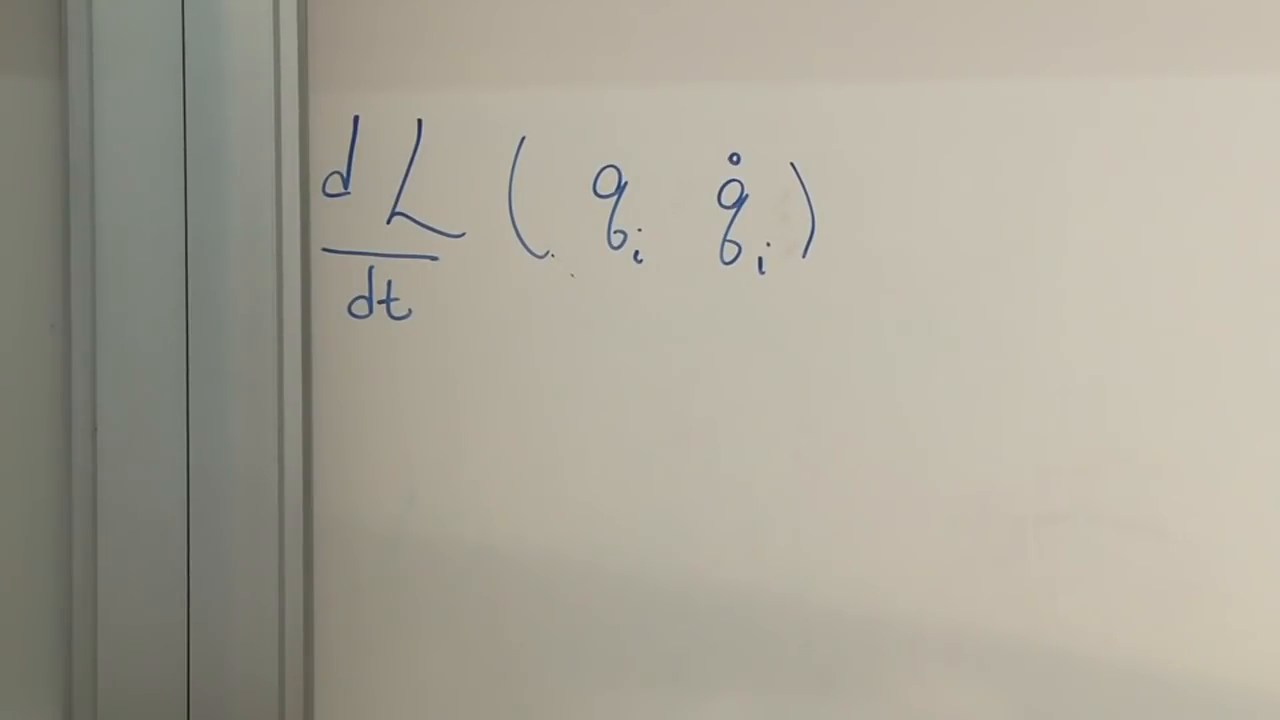
\includegraphics[width=0.72\textwidth]{lecture_05_figure_02.png}\caption{Inicio de la derivada de \(L(q_i,\dot q_i)\) a lo largo de la trayectoria.}\lectureframe{01:08:51}\end{figure}

\begin{classroomqa}\audiencequestion{¿Falta una sumatoria en la expresión de la regla de la cadena?\lecturetimestamp{01:10:39--01:11:05}}\lecturerresponse{Sí. Cualquier coordenada y cualquier velocidad pueden cambiar el Lagrangiano, así que se suman ambos términos sobre \(i\).}\end{classroomqa}

Utilicemos el momento canónico y la ecuación de Euler--Lagrange: \begin{equation}
  p_i=\frac{\partial L}{\partial\dot q_i},
  \qquad
  \dot p_i=\frac{\partial L}{\partial q_i}.
  \label{eq:l5-p-and-pdot}
\end{equation}. Entonces, la ec.~\eqref{eq:l5-chain-rule-no-time} se convierte en \begin{align}
  \frac{dL}{dt}
  &=\sum_i(\dot p_i\dot q_i+p_i\ddot q_i)
  \notag\\
  &=\frac{d}{dt}\sum_i p_i\dot q_i.
  \label{eq:l5-product-rule}
\end{align}. La ``magia'' no es más que la regla del producto.

\begin{figure}[htbp]\centering
  \includegraphics[width=0.84\textwidth]{lecture_05_figure_21.png}\caption{La regla de la cadena, convertida mediante las ecuaciones de movimiento en la derivada de \(\sum_i p_i\dot q_i\).}\lectureframe{01:13:45}\end{figure}

\begin{classroomqa}\audiencequestion{¿El último \(q_i\) del producto debería llevar uno o dos puntos encima?\lecturetimestamp{01:14:31--01:15:32}}\lecturerresponse{Dentro del producto es \(p_i\dot q_i\), con un solo punto. Al derivar el producto se obtiene \(\dot p_i\dot q_i+p_i\ddot q_i\), lo que explica los dos puntos del segundo término desarrollado.}\end{classroomqa}

Al restar las dos derivadas se obtiene una combinación conservada. Por convención histórica, se elige su opuesta y se la llama Hamiltoniano: \begin{equation}
  H=\sum_i p_i\dot q_i-L.
  \label{eq:l5-hamiltonian-definition}
\end{equation}

\begin{figure}[htbp]\centering
  \includegraphics[width=0.80\textwidth]{lecture_05_figure_22.png}\caption{La combinación conservada \(L-\sum_i p_i\dot q_i=-H\) y la definición del Hamiltoniano.}\lectureframe{01:18:05}\end{figure}

Para una partícula en un potencial, \begin{equation}
  L=\frac12m\dot x^2-V(x),
  \qquad p=m\dot x.
  \label{eq:l5-particle-lagrangian}
\end{equation}. Por tanto, \begin{align}
  H&=p\dot x-L
  \notag\\
   &=m\dot x^2-\left(\frac12m\dot x^2-V(x)\right)
  \notag\\
   &=\frac12m\dot x^2+V(x)=T+V.
  \label{eq:l5-particle-energy}
\end{align}.

\begin{figure}[htbp]\centering
  \includegraphics[width=0.86\textwidth]{lecture_05_figure_23.png}\caption{El Hamiltoniano de una partícula en un potencial se reduce a la conocida suma de las energías cinética y potencial.}\lectureframe{01:20:50}\end{figure}

La derivación no supuso ninguna forma particular para \(L\). Por tanto, la ec.~\eqref{eq:l5-hamiltonian-definition}, y no \(T+V\), es la definición general de energía en este formalismo.

\section{Dependencia explícita del tiempo e intercambio de energía}

Restablezcamos la dependencia explícita del tiempo en la regla de la cadena: \begin{equation}
  \frac{dL}{dt}
  =\sum_i\left(
    \frac{\partial L}{\partial q_i}\dot q_i
    +\frac{\partial L}{\partial\dot q_i}\ddot q_i
  \right)
  +\frac{\partial L}{\partial t}.
  \label{eq:l5-full-chain-rule}
\end{equation}. El lado izquierdo es la derivada total a lo largo del movimiento. En la derivada parcial final se mantienen fijos \(q\) y \(\dot q\) y se deriva únicamente respecto de los parámetros externos que cambian. Al repetir el mismo paso con la regla del producto se obtiene \begin{equation}
  \boxed{\frac{dH}{dt}=-\frac{\partial L}{\partial t}}.
  \label{eq:l5-hamiltonian-time}
\end{equation}.

\begin{figure}[htbp]\centering
  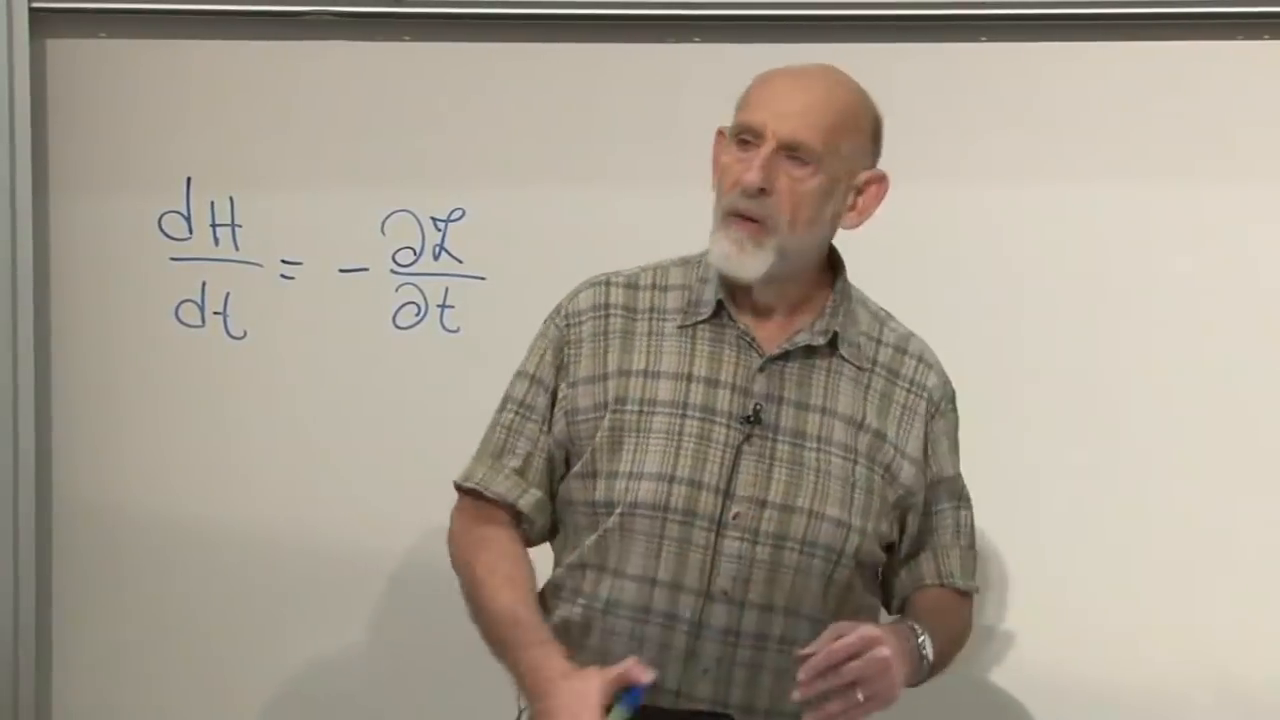
\includegraphics[width=0.70\textwidth]{lecture_05_figure_04.png}\caption{El Hamiltoniano solo cambia a través de la dependencia explícita del tiempo del Lagrangiano.}\lectureframe{01:37:22}\end{figure}

Para el oscilador sometido a una excitación externa de la ec.~\eqref{eq:l5-driven-oscillator}, \begin{equation}
  \frac{\partial L}{\partial t}
  =-\frac12\dot k(t)x^2,
  \qquad
  \dot H=\frac12\dot k(t)x^2.
  \label{eq:l5-driven-energy-rate}
\end{equation}. En \(x=0\), la tasa instantánea se anula; fuera del origen, cambiar la constante elástica realiza trabajo a una tasa proporcional a \(x^2\dot k\).

\begin{classroomqa}\audiencequestion{Si la energía no se conserva, ¿su definición es la derivada temporal del Hamiltoniano?\lecturetimestamp{01:27:11--01:28:04}}\lecturerresponse{No. La energía es \(H\). Su derivada nos indica cómo cambia esa energía. Cuando el Lagrangiano tiene la forma familiar, \(H=T+V\); cuando no la tiene, la ec.~\eqref{eq:l5-hamiltonian-definition} proporciona la definición. Ampliar el sistema para incluir el agente externo restablece la conservación del Hamiltoniano total.}\end{classroomqa}

\begin{classroomqa}\audiencequestion{¿Cómo se aplica esto al observador anterior situado en un tiovivo en rotación, donde aparecían términos centrífugos y de Coriolis?\lecturetimestamp{01:28:08--01:29:52}}\lecturerresponse{Un sistema de coordenadas que rota uniformemente implica un cambio de variables dependiente del tiempo, no una simetría espacial fija ni una simple traslación temporal. Su Lagrangiano transformado puede usarse para construir un Hamiltoniano, pero es mejor posponer ese cálculo aparte hasta que se traten las fuerzas magnéticas, ya que el álgebra tiene una forma estrechamente relacionada.}\end{classroomqa}

\section{El conjunto de herramientas lagrangianas de un vistazo}

Ahora podemos expresar toda la estructura en una secuencia compacta: \begin{align}
  L&=L(q_i,\dot q_i,t),
  \notag\\
  p_i&=\frac{\partial L}{\partial\dot q_i},
  \qquad
  \dot p_i=\frac{\partial L}{\partial q_i},
  \notag\\
  \delta q_i&=\epsilon f_i(q)
  \quad\Longrightarrow\quad
  Q=\sum_i p_i f_i(q),\quad \dot Q=0,
  \notag\\
  H&=\sum_i p_i\dot q_i-L,
  \qquad
  \dot H=-\frac{\partial L}{\partial t}.
  \label{eq:l5-toolkit}
\end{align}

\begin{figure}[htbp]\centering
  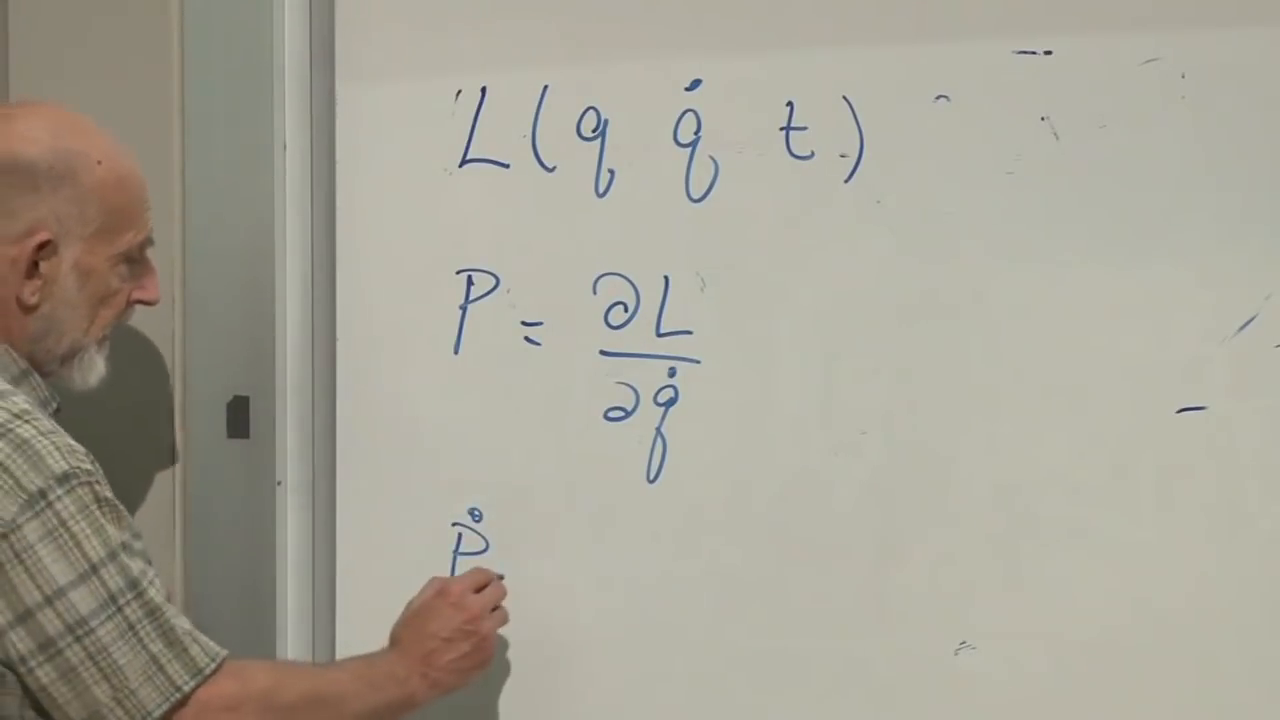
\includegraphics[width=0.66\textwidth]{lecture_05_figure_03.png}\caption{El repaso en la pizarra comienza con \(L(q,\dot q,t)\), el momento canónico y la ecuación de Euler--Lagrange.}\lectureframe{01:31:37}\end{figure}

Estas fórmulas contienen una definición, ecuaciones de movimiento, la carga de una simetría continua ordinaria y la carga de las traslaciones temporales. Hay pocos trucos; lo importante es poder volver a derivarlas, en vez de memorizar expresiones inconexas.

\section{¿Por qué usar la mecánica lagrangiana o hamiltoniana?}

\begin{classroomqa}\audiencequestion{¿Puede describirse la mecánica indistintamente con \(L\) o \(H\), y por qué elegir una formulación?\lecturetimestamp{01:37:16--01:39:18}}\lecturerresponse{Son equivalentes cuando la transformación de Legendre es regular, pero destacan estructuras distintas. El Lagrangiano parte de manera natural del principio de acción estacionaria. La mecánica hamiltoniana resulta más abstracta al principio, pero sus ecuaciones son sencillas y adquiere un papel central en la mecánica cuántica. El Hamiltoniano es la energía, pero su función va mucho más allá de la ley de conservación por sí sola.}\end{classroomqa}

\begin{classroomqa}\audiencequestion{¿Conocía Newton la forma hamiltoniana de la conservación de la energía?\lecturetimestamp{01:39:29--01:39:56}}\lecturerresponse{No en esta formulación, hasta donde indica el registro histórico. El marco que Newton enunció era la ley de fuerzas \(F=ma\).}\end{classroomqa}

\begin{classroomqa}\audiencequestion{¿Por qué debería todo sistema físico tener un Lagrangiano? ¿Es eso solo un hecho experimental?\lecturetimestamp{01:39:57--01:42:37}}\lecturerresponse{Para los sistemas cerrados que estamos considerando, es un hecho empírico y también se desprende de la descripción cuántica más profunda. Se pueden inventar ecuaciones diferenciales matemáticamente coherentes que no sean ecuaciones de Euler--Lagrange. Por ejemplo, \(\dot x=-x\) es perfectamente resoluble, pero, como ley fundamental cerrada de una coordenada, tiene el carácter disipativo de una pérdida de información. La mecánica clásica no precede lógicamente a la mecánica cuántica; hereda de esta su estructura fundamental. La razón detallada tendrá que esperar.}\end{classroomqa}

\begin{classroomqa}\audiencequestion{Si todo sistema cerrado real tiene un Lagrangiano, ¿corresponde toda función que llamamos Lagrangiano a algún sistema que se encuentre en la naturaleza?\lecturetimestamp{01:42:39--01:42:54}}\lecturerresponse{No. El cálculo formal admite muchas funciones que no se realizan en ningún sistema físico conocido.}\end{classroomqa}

\begin{classroomqa}\audiencequestion{¿Es el Lagrangiano principalmente una herramienta para inventar potenciales?\lecturetimestamp{01:42:54--01:43:32}}\lecturerresponse{Es más amplio que eso. Puede servir para organizar sistemas mecánicos candidatos y, a menudo, es la vía práctica más breve para obtener las ecuaciones de movimiento.}\end{classroomqa}

El péndulo doble muestra esa ventaja práctica. Se eligen dos ángulos, se calculan las velocidades de ambas masas en función de esos ángulos y sus derivadas temporales, se forma \(T-V\) y se deja que las ecuaciones de Euler--Lagrange tengan en cuenta implícitamente las fuerzas de vínculo. Es mucho más sencillo que calcular todas las tensiones y aceleraciones con \(F=ma\).

\begin{figure}[htbp]\centering
  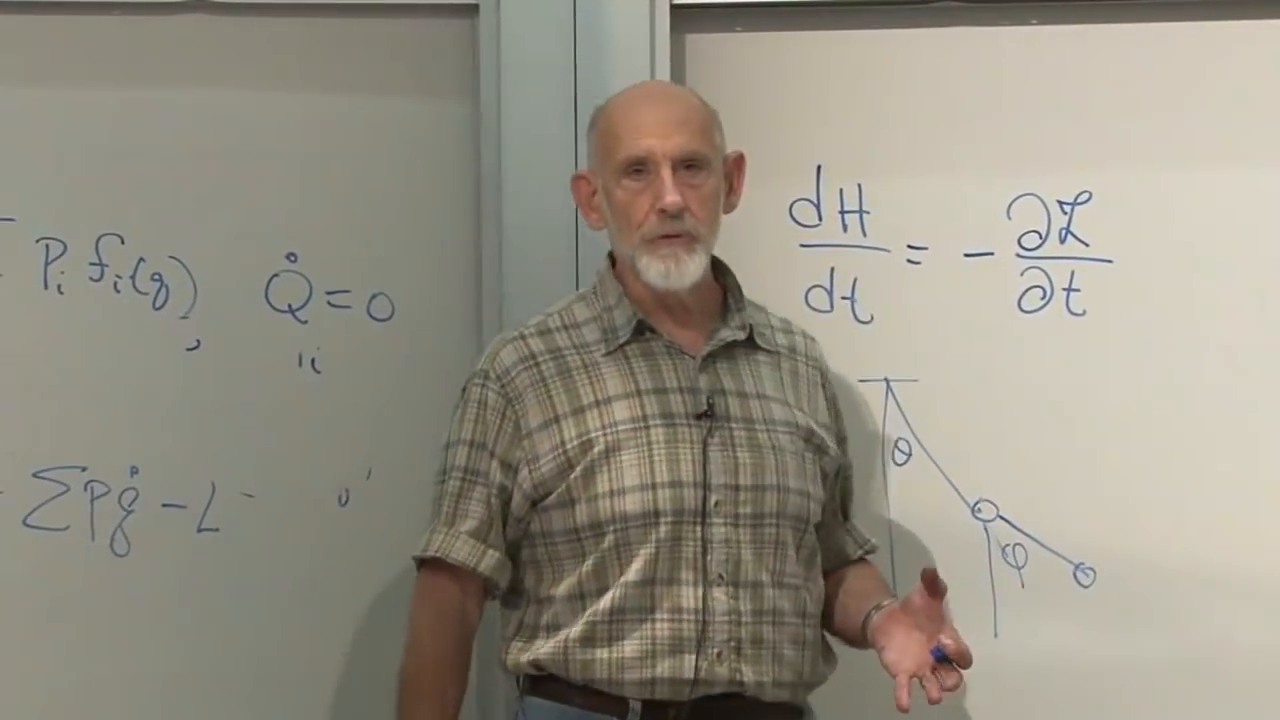
\includegraphics[width=0.84\textwidth]{lecture_05_figure_05.png}\caption{La identidad de la tasa de cambio de la energía permanece en la pizarra junto al esquema del péndulo doble.}\lectureframe{01:45:39}\end{figure}

\begin{figure}[htbp]\centering
  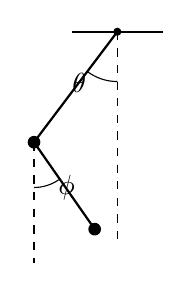
\begin{tikzpicture}[scale=1.15]
    \draw[thick] (-0.5,0) -- (0.5,0);
    \fill (0,0) circle (0.045);
    \draw[dashed] (0,0) -- (0,-2.3);
    \draw[thick] (0,0) -- (-0.92,-1.22);
    \fill (-0.92,-1.22) circle (0.07);
    \draw[dashed] (-0.92,-1.22) -- (-0.92,-2.55);
    \draw[thick] (-0.92,-1.22) -- (-0.25,-2.18);
    \fill (-0.25,-2.18) circle (0.07);
    \draw (0,-0.55) arc (-90:-127:0.55);
    \node at (-0.42,-0.56) {$\theta$};
    \draw (-0.92,-1.72) arc (-90:-55:0.48);
    \node at (-0.56,-1.72) {$\phi$};
  \end{tikzpicture}\caption{Coordenadas angulares generalizadas para un péndulo doble.}\end{figure}

Cambiar de variables resulta igual de eficaz: se transforma un Lagrangiano y luego se derivan sus ecuaciones, en lugar de transformar por separado cada ecuación de fuerzas.

\begin{classroomqa}
  \audiencequestion{¿Es el péndulo doble, en esencia, otro sistema de tres cuerpos, como el formado por el Sol, la Tierra y la Luna, en el que uno de los cuerpos se trata como anclaje?
  \lecturetimestamp{01:45:06--01:45:25}}
  \lecturerresponse{La analogía refleja esa jerarquía, aunque las varillas imponen restricciones distintas. En ambos casos, en una aproximación, puede tratarse un componente muy masivo o fijo como estructura de referencia.}
\end{classroomqa}

\begin{classroomqa}
  \audiencequestion{En el péndulo doble se usa \(T-V\), aunque acabamos de hacer hincapié en que hay lagrangianos más generales. ¿Cuándo es válida \(T-V\)?
  \lecturetimestamp{01:46:08--01:46:58}}
  \lecturerresponse{La forma habitual se aplica a partículas no relativistas ordinarias observadas en un sistema de referencia inercial, sin acoplamiento magnético con la velocidad. Los sistemas de referencia en rotación, los sistemas relativistas y los campos magnéticos requieren términos más generales.}
\end{classroomqa}

\begin{classroomqa}
  \audiencequestion{¿Quedan las colisiones fuera de esta descripción?
  \lecturetimestamp{01:47:00--01:48:05}}
  \lecturerresponse{Las colisiones elásticas se deben a fuerzas de corto alcance y, por tanto, a potenciales. A nivel microscópico, las colisiones inelásticas siguen siendo mecánicas, pero la energía pasa a vibraciones internas, deformación y calor. Una descripción del centro de masas que omita esos grados de libertad es incompleta.}
\end{classroomqa}

\begin{classroomqa}
  \audiencequestion{¿Se puede analizar una pelota de béisbol golpeada por un bate mediante \(F=ma\)?
  \lecturetimestamp{01:48:05--01:48:33}}
  \lecturerresponse{Solo a grandes rasgos. Para dar cuenta de todo hay que seguir la deformación, el calentamiento, los posibles daños a la pelota y quizá la rotura del bate. Esos grados de libertad internos explican por qué un impacto realista es mucho más difícil de analizar que una colisión entre partículas puntuales.}
\end{classroomqa}

\begin{classroomqa}
  \audiencequestion{¿Y qué ocurre con un cuerpo rígido extenso?
  \lecturetimestamp{01:48:34--01:49:00}}
  \lecturerresponse{Los cuerpos rígidos pueden estudiarse con métodos newtonianos o mediante un lagrangiano \(T-V\) expresado en coordenadas de traslación y rotación. Construir ese lagrangiano es un ejercicio útil.}
\end{classroomqa}

\begin{classroomqa}
  \audiencequestion{¿Significa la relación de incertidumbre entre energía y tiempo de la mecánica cuántica-- que la energía no se conserva estrictamente?
  \lecturetimestamp{01:49:01--01:49:29}}
  \lecturerresponse{No. La energía puede conservarse estrictamente. La relación indica que, para determinar la energía con gran precisión, hay que observar durante mucho tiempo; no sustituye la ley de conservación.}
\end{classroomqa}

\begin{classroomqa}
  \audiencequestion{¿Son lógicamente equivalentes la mecánica newtoniana y la lagrangiana?
  \lecturetimestamp{01:49:36--01:50:07}}
  \lecturerresponse{Son equivalentes en el dominio habitual en el que se aplican ambas formulaciones. Aun así, se pueden inventar lagrangianos cuyas ecuaciones no se parezcan a la forma elemental \(m\ddot x=F(x)\).}
\end{classroomqa}

\section{Un término cinético dependiente de la coordenada}

Consideremos el siguiente ejemplo, deliberadamente poco familiar:
\begin{equation}
  L=\frac12q^2\dot q^2-\frac12q^2.
  \label{eq:l5-nonstandard-l}
\end{equation}
Es un lagrangiano válido con un coeficiente cinético dependiente de la coordenada. También se pueden considerar términos lineales en la velocidad, como \(q\dot q\); en este ejemplo unidimensional, ese término en particular es una derivada total y no modificaría las ecuaciones de movimiento.

El momento canónico es
\begin{equation}
  p=\frac{\partial L}{\partial\dot q}=q^2\dot q,
  \label{eq:l5-nonstandard-p}
\end{equation}
por lo que
\begin{equation}
  \dot p=q^2\ddot q+2q\dot q^2,
  \qquad
  \frac{\partial L}{\partial q}=q\dot q^2-q.
  \label{eq:l5-nonstandard-derivatives}
\end{equation}
La ecuación de movimiento es, por tanto,
\begin{equation}
  q^2\ddot q+q\dot q^2=-q.
  \label{eq:l5-nonstandard-eom}
\end{equation}

\begin{figure}[htbp]
  \centering
  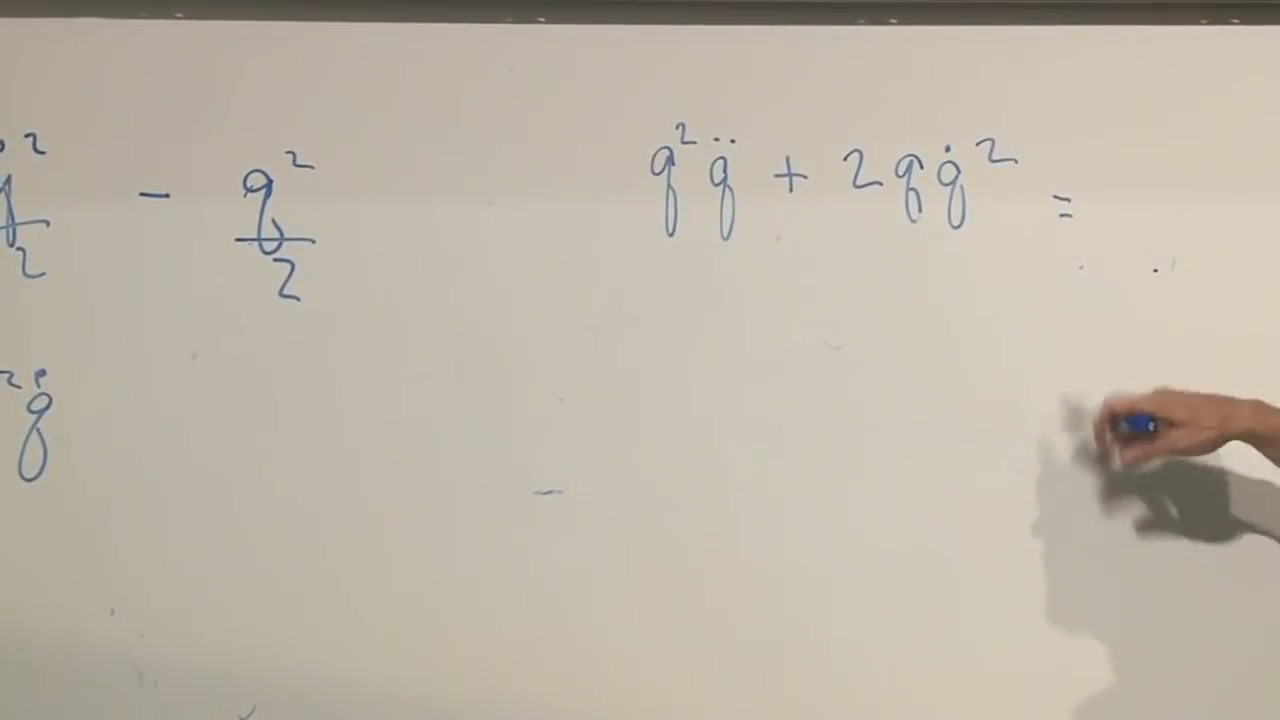
\includegraphics[width=0.80\textwidth]{lecture_05_figure_06.png}
  \caption{El momento derivado en el ejemplo con un término cinético dependiente de la coordenada.}
  \lectureframe{01:52:32}
\end{figure}

\begin{classroomqa}
  \audiencequestion{¿Se puede dividir la ecuación por \(q\)?
  \lecturetimestamp{01:53:22--01:53:39}}
  \lecturerresponse{Solo cuando \(q\neq0\). En \(q=0\), el coeficiente cinético y la aplicación de Legendre son degenerados, por lo que dividir descartaría un punto singular que requiere un tratamiento aparte.}
\end{classroomqa}

El hamiltoniano es
\begin{align}
  H&=p\dot q-L
  \notag\\
   &=q^2\dot q^2-
     \left(\frac12q^2\dot q^2-\frac12q^2\right)
  \notag\\
   &=\frac12q^2\dot q^2+\frac12q^2.
  \label{eq:l5-nonstandard-h}
\end{align}

\begin{classroomqa}
  \audiencequestion{¿Se puede seguir llamando energía cinética a \(q^2\dot q^2/2\)?
  \lecturetimestamp{01:54:41--01:55:07}}
  \lecturerresponse{Sí. En este ejemplo desarrollado, el hamiltoniano vuelve a tener la forma de un término cinético positivo más un término potencial. La idea es que las definiciones formales funcionan sin suponer de antemano la forma elemental de masa constante.}
\end{classroomqa}

\section{Disipación y el origen más profundo del formalismo}

\begin{classroomqa}
  \audiencequestion{¿Cómo se incluye la fricción en un lagrangiano?
  \lecturetimestamp{01:55:09--01:56:17}}
  \lecturerresponse{No se incluye como fuerza fundamental en el sistema cerrado sencillo con un número finito de grados de libertad que consideramos aquí. La fricción macroscópica es un efecto estadístico de cantidades enormes de grados de libertad microscópicos. Esos átomos siguen obedeciendo la mecánica subyacente, pero una descripción reducida que no los siga muestra disipación.}
\end{classroomqa}

\begin{classroomqa}
  \audiencequestion{¿Cómo llegó Hamilton a su formulación?
  \lecturetimestamp{01:56:22--01:56:37}}
  \lecturerresponse{Aquí no se ha presentado ninguna derivación histórica. La tarea importante para este curso es entender cómo funciona la formulación.}
\end{classroomqa}

\begin{classroomqa}
  \audiencequestion{¿Hay un procedimiento más general para obtener un lagrangiano cuando no tiene a simple vista la forma \(T-V\)?
  \lecturetimestamp{01:56:43--01:58:54}}
  \lecturerresponse{La función puede obtenerse mediante experimentos, una conjetura fundamentada, un principio de simetría o la reconstrucción a partir de las ecuaciones deseadas. Preguntarse de dónde obtiene su entrada el cálculo es como preguntarse de dónde salió \(f(x)\) en la definición de derivada. El cálculo nos dice qué hacer una vez especificada la función. La mecánica cuántica responde, en un nivel más profundo, por qué los sistemas cerrados de la naturaleza se ajustan a esta estructura abstracta.}
\end{classroomqa}

Este punto conecta con los temas iniciales del curso. La evolución hamiltoniana fundamental es determinista y reversible, en el sentido de que las trayectorias no se fusionan y la información no se destruye sin más. La relación entre esa propiedad y la formulación en el espacio de fases se desarrollará por etapas.

\begin{classroomqa}
  \audiencequestion{¿El cálculo variacional simplemente trabajó hacia atrás, partiendo de las ecuaciones clásicas deseadas, y obtiene la mecánica cuántica su lagrangiano del mismo modo?
  \lecturetimestamp{01:59:37--02:01:07}}
  \lecturerresponse{En la construcción clásica elemental, efectivamente se puede elegir una acción cuyas trayectorias estacionarias reproduzcan las ecuaciones conocidas. En mecánica cuántica, el orden lógico es distinto: se parte de forma natural del hamiltoniano y se puede llegar a una descripción lagrangiana. Allí el hamiltoniano resulta más intuitivo, aunque en mecánica clásica aparezca primero como algo abstracto.}
\end{classroomqa}

\begin{classroomqa}
  \audiencequestion{¿Puede la mecánica cuántica describir la fricción?
  \lecturetimestamp{02:01:08--02:02:05}}
  \lecturerresponse{Sí, pero una descripción fundamental debe incluir los grados de libertad del entorno. No se puede describir por completo una partícula que se mueve en un fluido viscoso sin incluir las partículas del fluido. La fricción es el complicado efecto colectivo que emerge cuando esos grados de libertad no se siguen individualmente.}
\end{classroomqa}
